% This text is Free and open Open Source.
% It's a part of presentation made by myself.
% It may be used only for academic purpose
% May, 2012
% Author: Seshagiri Prabhu
% Amrita Vishwa Vidyapeethm 
% seshagiriprabhu@gmail.com
% www.seshagiriprabhu.wordpress.com

\documentclass[12pt]{beamer}
\usetheme{Oxygen}
\usepackage{thumbpdf}
\usepackage{wasysym}
\usepackage{ucs}
\usepackage[utf8]{inputenc}
\usepackage{pgf,pgfarrows,pgfnodes,pgfautomata,pgfheaps,pgfshade}
\usepackage{verbatim}
\usepackage{listings}
\usepackage{courier}
\usepackage{caption}
\usepackage{verbatim} 
\usepackage{upquote}
\usepackage{graphics}
\usepackage{latexsym}
\usepackage{fixltx2e}
\usepackage{hyperref}
\usepackage{amssymb}

\usepackage{pgf}
\usepackage{fmtcount}% http://ctan.org/pkg/fmtcount
\usepackage{algorithm, algpseudocode}
\usepackage{caption}
\captionsetup[algorithm]{font=scriptsize}
\usepackage{lipsum}
\usepackage{float}
\setbeamerfont{caption}{size=\footnotesize}

\newcommand\Fontvi{\fontsize{5}{6}\selectfont}
%\renewcommand\tinyv{\@setfontsize\tinyv{4pt}{6}}
%\renewcommand\tiny{\@setfontsize\tiny{4pt}{6}}

\usepackage{xcolor}
\def\SPSB#1#2{\rlap{\textsuperscript{\textcolor{red}{#1}}}\SB{#2}}
\def\SP#1{\textsuperscript{\textcolor{red}{#1}}}
\def\SB#1{\textsubscript{\textcolor{blue}{#1}}}

\pdfinfo
{
  /Title       (Stealth File Systems  for Proactive Forensics Support in Custom Android ROMs)
  /Creator     (Sudip Hazra)
  /Author      (TeX)
}


\title{Stealth File Systems  for Proactive Forensics Support in Custom Android ROMs}

% A subtitle is optional and this may be deleted
%\subtitle{Optional Subtitle}

\author{Guide: Dr. Prabhakar Mateti\inst{1} \and Sudip Hazra\inst{2}}
% - Give the names in the same order as the appear in the paper.
% - Use the \inst{?} command only if the authors have different
%   affiliation.

\institute[Universities of Somewhere and Elsewhere] % (optional, but mostly needed)
{
  \inst{1}%
  Wright State University
  \and
  \inst{2}%
  Amrita Centre For Cyber Security Systems and Networks\\
 Amrita University}
% - Use the \inst command only if there are several affiliations.
% - Keep it simple, no one is interested in your street address.

\date{12 December 2016}
% - Either use conference name or its abbreviation.
% - Not really informative to the audience, more for people (including
%   yourself) who are reading the slides online

\subject{Theoretical Computer Science}
% This is only inserted into the PDF information catalog. Can be left
% out. 

% If you have a file called "university-logo-filename.xxx", where xxx
% is a graphic format that can be processed by latex or pdflatex,
% resp., then you can add a logo as follows:

% \pgfdeclareimage[height=0.5cm]{university-logo}{university-logo-filename}
% \logo{\pgfuseimage{university-logo}}

% Delete this, if you do not want the table of contents to pop up at
% the beginning of each subsection:
\AtBeginSubsection[]
{
  \begin{frame}<beamer>{Outline}
    \tableofcontents[currentsection,currentsubsection]
  \end{frame}
}

% Let's get started
\begin{document}

\begin{frame}
  \titlepage
 
\end{frame}

\begin{frame}{Outline}
  \tableofcontents
 
  % You might wish to add the option [pausesections]
\end{frame}

% Section and subsections will appear in the presentation overview
% and table of contents.
\section{Introduction}
\subsection{Why Mobile Forensics}
\centering
\vspace{5cm}
\bf{Smartphone OS Market}
\begin{figure}
\vspace{-1cm}
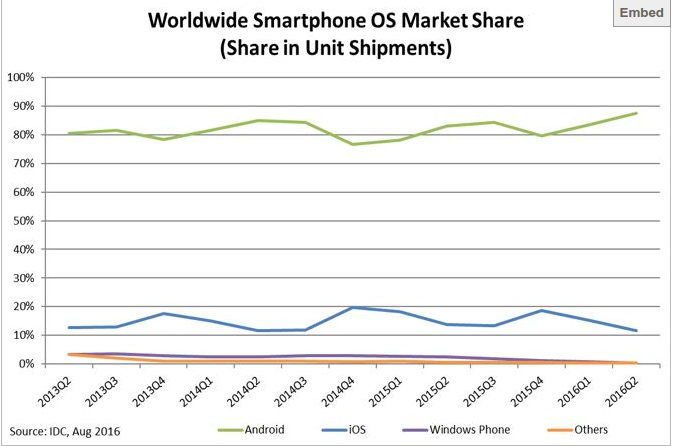
\includegraphics[width=8cm,height=5cm]{images/idc}
%\caption{Smartphone OS Market Share, 2016 Q2}
\end{figure}
\begin{frame}{Why Mobile Forensics Is Important}
Just from cell phones, a mobile phone forensic analysis can reveal a great deal of data, including:
\begin{itemize}
\item Dialed, incoming and missed calls (history logs)
\item Text messages
\item Instant message activity
\item Email
\item Internet activity including search histories
\item Video and audio recordings
\item Phone location information (using GPS) and cell phone tower triangulation
\end{itemize}
  
\end{frame}












































\section{Background}

\subsection{Forensic Rom}
\begin{frame}{Forensic Rom}{Work Done Till Now}
  \begin{itemize}
  \item {
   Features of  Aiyappan Et.al \cite{Aiyappan} and Karthik Et.al \cite{Karthik} Forensic Rom:
   
   \bigskip
   \item{
   Captures All User Activities.}
   
   \bigskip 
   \item{
   Key-logging and Call Tapping Facility.}
   
   \bigskip
   \item{
   Opportunistically Uploads In Cloud.}
   
   \bigskip
   \item{
   Hiding the Process using hidepid =2.
}

	\bigskip
   \item{
   Data Stored in /forensic partition only accessible to Root.}
   
   
  }
  
  
  \end{itemize}
\end{frame}
\subsection{Shortfalls}
\begin{frame}{Shortfalls}

	\begin{itemize}
	
	\item{
	
	What if The Suspect Roots the Phone ?
	}
	\bigskip
	\item{
	
		Can Find the /forensic Partition.	
	}	
	\end{itemize}





\end{frame}

\subsection{Possible Solutions}
\begin{frame}{Posible Solutions}
	\begin{itemize}
	\item{
	Encrypting The /forensic partition can Still arise Suspicion.
	}
	\bigskip
	\item{
	Creating A Fuse File System and enable Stealth Features and Copy all Forensically Relevant Data in that File System.
	
	}
	\end{itemize}
\end{frame}


\section{Proposed Framework}

\subsection{File System in User Space}
\begin{frame}{File System in User Space}
\begin{itemize}
\item{
The Filesystem in Userspace (FUSE) is a special part of the Linux \indent kernel that \indent allows regular users to make and use their own file-systems \indent without needing to change the kernel or have Root privileges.
}


\end{itemize}
\end{frame}

\subsection{Linux Cloud Drive}
\begin{frame}{Linux Cloud Drive}
	\begin{itemize}
	\item{Using FUSE we can mount Cloud Drive in Our System and Use it Like a Local File System.
	}
	\bigskip
	
	 \item \href{https://github.com/GoogleCloudPlatform/gcsfuse}{Gcsfuse:} A user-space file system for interacting with Google Cloud Storage.
	 \bigskip
	 
	 \item \href{http://www.archiware.com/products/wingfs}{Wingfs:} A debian Package to mount various cloud storage drives as user-space file systems.
	 \bigskip 
	 \item \href{https://ahmetalpbalkan.com/blog/introducing-azurefs/}{Azurefs:} A python package to mount Azure blob storage as Local File system.
	 \end{itemize}	   	
\end{frame}
\subsection{Android Rootkits}
\begin{frame}{Android Rootkits}
	\begin{itemize}
	\item Dong-Hoon Et.al \cite{Dong} has listed the various ways Rootkits can infect Android Kernel Like:
	\bigskip
	\begin{itemize}
	\item sys\_call\_table hooking through /dev/kmem access technique.
	\bigskip
	\item exception vector table modifying hooking techniques.
	
	\end{itemize}
	
	\item Our Objective is to Make the /Forensic Partition a Fuse File system and Hide it using Rootkits.
		
	\end{itemize}
\end{frame}

\subsection{Stealth File Systems}
\begin{frame}{Stealth File Systems }{Proposed Framework}

\end{frame}


\begin{frame}{Summary}
\begin{block}{Summary}
This Framework can effectively Hide the forensic as well as the cloud file system so that even if the Suspect is connecting to adb to check the internal state , He will not be able to find the  hidden File systems.
\end{block}


\end{frame}

% Placing a * after \section means it will not show in the
% outline or table of contents.
\section*{Summary}

\begin{frame}{Summary}
  \begin{itemize}
  \item
    \alert{Process Hiding} can also be Implemented Using this Technique
  \item
    The \alert{Stealth File-system}  will periodically copy the forensically relevant data from the normal file system
  \item This data will be moved to the \alert{Mounted Cloud Drive} and opportunistically uploaded to the cloud server. 
  \end{itemize}
  
  \begin{itemize}
  \item
    Outlook
    \begin{itemize}
    \item
     
     Have Developed a High-Level Overview of the Framework.
    \item
      Implementation Needs to be done.
    \end{itemize}
  \end{itemize}
\end{frame}



% All of the following is optional and typically not needed. 
\appendix
\section<presentation>*{\appendixname}
\subsection<presentation>*{Reference}

\begin{frame}[allowframebreaks]
  \frametitle<presentation>{References}
  
  \begin{thebibliography}{10}
  \bibitem{Aiyappan} 
  \textit{Android forensic support framework},
  Aiyappan.P
  Advisor:Prabhaker Mateti,
  M.Tech thesis, Amrita
  Vishwa Vidyapeetham,2015
   
  \bibitem{Karthik} 
  \textit{Proactive Forensic Support for Android Devices},
  Karthik K. 
  Advisor:Prabhaker Mateti
  M.Tech thesis,
  Amrita Vishwa Vidyapeetham,2016 
  
  \bibitem{Dong}
    \textit{Android platform based linux kernel rootkit},
    Dong-Hoon You, Bong-Nam Noh,
    Malicious and Unwanted Software (MALWARE), 2011 6th International Conference ,IEEE
    
    
    
    
    
 
  
   
 
  \end{thebibliography}
  
  
   
\end{frame}


\end{document}
